\documentclass{training}
\setlang{french}
% Filigrane PAR MODULE : \uxfond (PNG A4 dilue 30 %). Cadre noir vectoriel commun.
% Proportions original 744 px : marge 20/744, trait 1/744. Exterieur BLANC.
% Cadre via eso-pic +\put (coordonnees absolues) — pas de remember picture (decalage).
\usepackage{eso-pic}

\providecommand{\uxfond}{../../resources/fond/norme_fond_paliers_30.png}

\newlength{\uxmargin}
\newlength{\uxthick}
\newlength{\uxinnerw}
\newlength{\uxinnerh}
\setlength{\uxmargin}{0.02688\paperwidth}% 20/744
\setlength{\uxthick}{0.001344\paperwidth}% 1/744
\setlength{\uxinnerw}{\dimexpr\paperwidth-2\uxmargin-2\uxthick\relax}
\setlength{\uxinnerh}{\dimexpr\paperheight-2\uxmargin-2\uxthick\relax}

% Contenu strictement a l'interieur du trait (+ jour confortable).
\geometry{%
  includeheadfoot,
  left=22mm,
  right=22mm,
  top=20mm,
  bottom=18mm,
  headheight=30pt,
  headsep=5mm,
  footskip=12mm%
}

\AddToShipoutPictureBG{%
  \AtPageLowerLeft{%
    % Fond blanc page entiere
    \put(0,0){\color{white}\rule{\paperwidth}{\paperheight}}%
    % Filigrane module a l'interieur du cadre
    \put(\LenToUnit{\dimexpr\uxmargin+\uxthick\relax},\LenToUnit{\dimexpr\uxmargin+\uxthick\relax}){%
      \includegraphics[width=\uxinnerw,height=\uxinnerh]{\uxfond}}%
    % Cadre noir : bas, haut, gauche, droite
    \put(\LenToUnit{\uxmargin},\LenToUnit{\uxmargin}){%
      \color{black}\rule{\dimexpr\paperwidth-2\uxmargin\relax}{\uxthick}}%
    \put(\LenToUnit{\uxmargin},\LenToUnit{\dimexpr\paperheight-\uxmargin-\uxthick\relax}){%
      \color{black}\rule{\dimexpr\paperwidth-2\uxmargin\relax}{\uxthick}}%
    \put(\LenToUnit{\uxmargin},\LenToUnit{\uxmargin}){%
      \color{black}\rule{\uxthick}{\dimexpr\paperheight-2\uxmargin\relax}}%
    \put(\LenToUnit{\dimexpr\paperwidth-\uxmargin-\uxthick\relax},\LenToUnit{\uxmargin}){%
      \color{black}\rule{\uxthick}{\dimexpr\paperheight-2\uxmargin\relax}}%
  }%
}

\makeatletter
\fancyhf{}
\fancyheadoffset{0pt}
\renewcommand{\headrulewidth}{0pt}
\lhead{\parbox[t]{0.56\textwidth}{\RaggedRight\footnotesize\sloppy\@title}}
\rhead{\parbox[t]{0.36\textwidth}{\RaggedLeft\footnotesize\sloppy\@subtitle}}
\cfoot{\thepage}
% Coupures : underscore et slash dans les noms de fichiers / consignes
\DeclareRobustCommand{\_}{\textunderscore\allowbreak}
\makeatother

% Evite les depassements de longues lignes (Github, Name_FirstName_...)
\sloppy
\emergencystretch=3em
\hbadness=10000

% Sommaire type 42 : chapitres seulement
\setcounter{tocdepth}{0}
\renewcommand{\cftchappresnum}{}
\renewcommand{\cftchapaftersnum}{}
\setlength{\cftchapnumwidth}{2.0em}
\setlength{\cftbeforechapskip}{0.35em}
\cftsetindents{chapter}{0em}{2.0em}


\begin{document}

\schoollogo{../../resources/jeunecrack.png}
\title{Music on}
\subtitle{Piscine UX/UI --- UX}
\member{Piscine UX/UI}{https://github.com/01-edu/UX-UI}
\summary{Heuristiques, carte, jobs to be done, tri, wireframes, tests.}
\version{1.0}
\prerequisite{Le module précédent de cette piscine, ou aucun si c'est le premier.}
\maketitle

\newpage
\tableofcontents
\newpage


\chapter{Instructions}

L'avant-propos n'est pas un exercice. Il ne sera pas noté. Les exercices commencent au chapitre suivant, du contrat le plus simple au plus dur. Un exercice plus tardif n'est pas pris en compte si un plus tôt ne tient pas.

On ne regarde que ce qui est dans le répertoire de rendu de l'exercice. N'ajoutez pas un fichier que l'exercice ne nomme pas. Le nom d'un livrable suit le motif imprimé dans l'exercice : \texttt{Name\_FirstName\_DeliverableName\_Date\_VersionNumber}.

Le geste ne vous est pas donné. Les exemples d'un exercice portent parfois une contrainte que la phrase ne répète pas. Lisez-les. Vos autres références sont le manuel de l'outil choisi, la personne assise à côté, et les liens imprimés dans l'exercice.

L'ordre est celui de la quête. Sauter une étape parce qu'un écran plus tard semble plus intéressant produit un écran que personne ne sait expliquer.

\subsection*{Des images}

La marque en couverture est le logo du projet. L'image de l'avant-propos est l'illustration de ce module. Le fond pâle derrière le texte est le filigrane de page. Aucun n'est un indice.

\subsection*{Des machines qui écrivent}

Vous pouvez vous servir d'un outil pour vérifier un mot, comme d'un dictionnaire. Vous ne pouvez pas remplacer un entretien, un test ou un fichier par un texte généré et le signer. Si vous ne pouvez pas montrer la personne, l'écran ou la ligne que vous avancez, l'exercice n'est pas fait.


\chapter{Avant-propos}

Les pochettes de Paula Scher pour CBS Records sont fortes exprès : la pochette est la promesse, le morceau est la preuve. \emph{High Fidelity} (Stephen Frears, 2000) est l'autre moitié de la blague, un homme qui classe des disques parce que classer est sa façon de penser. Cette quête classe un service de musique. Le film n'est pas le tri de cartes.

\begin{center}
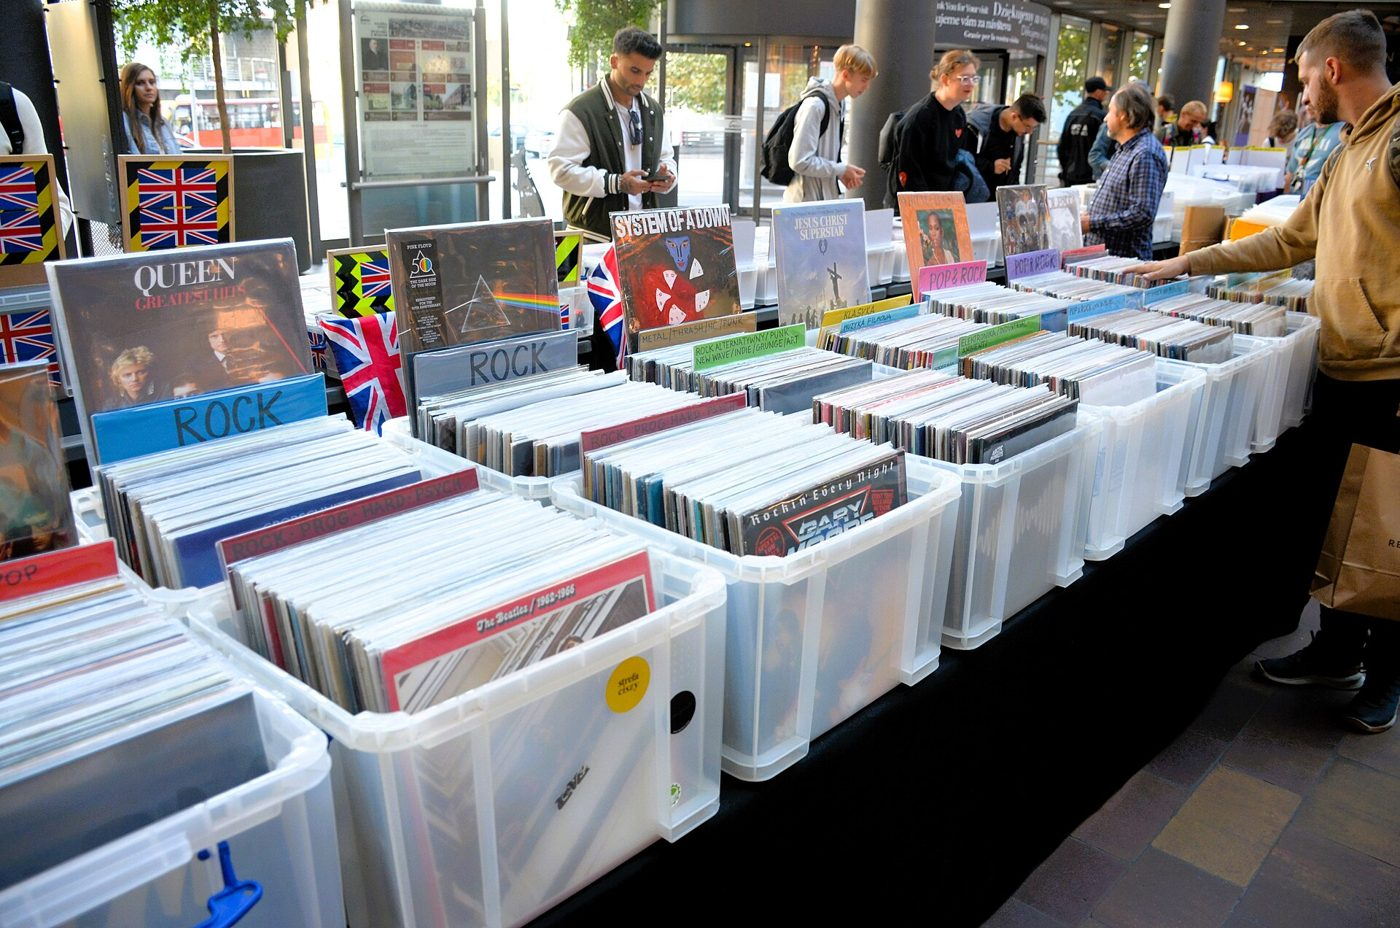
\includegraphics[width=0.78\textwidth,height=0.32\textheight,keepaspectratio]{../../resources/intros/UX-04-music-on.jpg}\\[0.4em]
{\footnotesize Image : Silar / CC BY-SA 4.0}
\end{center}

À regarder. Les vidéos sont un contexte. Elles ne sont pas le livrable.
\begin{itemize}
\item UX - Introduction \& Quest n°1, 01Edu \url{https://www.youtube.com/watch?v=UbE6WMeuvQg&list=PLHyAJ_GrRtf-RAtfngbRrFh1XDTnyXFDe}
\end{itemize}

\chapter{Exercice 00 : UX V - Ex 1 - Heuristiques}
\exnumber{00}
\extitle{UX V - Ex 1 - Heuristiques}
\exfiles{ex00/PDF, nomme Name\_FirstName\_DeliverableName\_Date\_VersionNumber}
\exauthorize{Ceux nommés dans l'exercice}
\makeheaderfiles

\textbf{Contexte :}

Un label musical spécialisé dans la musique d'Amérique du Sud vous demande d'améliorer l'expérience utilisateur. Cette quête porte sur les heuristiques et l'organisation du contenu !

\textbf{Instructions :}

Menez une analyse heuristique sur \textbf{un} de ces sites web :

\begin{itemize}
\item Universal Music Latin America \url{https://www.universalmusica.com/}
\item Delta Records \url{https://deltarecords.net/}
\item Zoho Music \url{https://www.zohomusic.com/}
\item Luaka Bop \url{https://www.luakabop.com/}
\item Rimas Music \url{https://rimasmusic.com/}
\item D'autres... tant que c'est un label de musique sud-américain ;-)
\end{itemize}

\textbf{Livrables :}

\begin{itemize}
\item Une checklist dupliquée et complétée sur un tableur (Google Sheets, Airtable, Excel, etc.)
\item Outil : checklist d'évaluation heuristique \url{https://drive.google.com/file/d/10KbfbNZA1oVS1sXbjjXLPPmdZ6nqVkdc/view}
\item Déposez le document sur Github, nommé comme suit : « Nom\_Prénom\_NomDuLivrable\_Date\_NumeroDeVersion ». Par exemple, cela peut être nommé « Doe\_John\_MidFiPrototype\_05242024\_V1 ».
\item Ajoutez un titre dans le document.
\item Soignez l'aspect global du document. Il doit être clair, simple et lisible. Vous pouvez regarder canva.com, sans surcharger le dessin de détails.
\end{itemize}

\textbf{Ressources :}

\begin{itemize}
\item 3 façons dont un bon design vous rend heureux - TED talk de Don Norman \url{https://www.ted.com/talks/don_norman_3_ways_good_design_makes_you_happy}
\item Introduction à l'évaluation heuristique : un guide pour débutants \url{https://uxdesign.cc/introduction-to-heuristic-evaluation-658705606518}
\item Les 10 heuristiques d'utilisabilité de Nielsen \url{https://www.nngroup.com/articles/ten-usability-heuristics/}
\item Ce que vous retirez vraiment d'une évaluation heuristique \url{https://uxmag.com/articles/what-you-really-get-from-a-heuristic-evaluation}
\item Analyse heuristique pour l'UX : comment mener une évaluation d'utilisabilité \url{https://uxdesign.cc/heuristic-analysis-for-ux-how-to-run-a-usability-evaluation-12c86d43936f}
\item L'analyse heuristique dans le processus de design \url{https://uxdesign.cc/heuristic-analysis-in-the-design-process-usability-inspection-methods-d200768eb38d}
\item Une nouvelle checklist d'évaluation heuristique d'utilisabilité \url{https://uxplanet.org/a-new-usability-heuristic-evaluation-checklist-259f588da308}
\end{itemize}

\textbf{Citation :}

« Si vous pensez que le design est cher, regardez le coût d'un mauvais design » Ralf Speth | Ancien PDG Jaguar Land Rover


\chapter{Exercice 01 : UX V - Ex 2 - Plan de site}
\exnumber{01}
\extitle{UX V - Ex 2 - Plan de site}
\exfiles{ex01/fichier Figma et PDF, nomme Name\_FirstName\_DeliverableName\_Date\_VersionNumber}
\exauthorize{Ceux nommés dans l'exercice}
\makeheaderfiles

\textbf{Instructions :}

Restez sur le site web que vous avez choisi dans l'Ex.1 et concevez un plan de site. Le plan de site doit inclure toutes les pages du site ainsi que les connexions et la hiérarchie.

\textbf{Liste de sites :}

\begin{itemize}
\item Universal Music Latin America \url{https://www.universalmusica.com/}
\item Delta Records \url{https://deltarecords.net/}
\item Zoho Music \url{https://www.zohomusic.com/}
\item Luaka Bop \url{https://www.luakabop.com/}
\item Rimas Music \url{https://rimasmusic.com/}
\item D'autres... tant que c'est un label de musique sud-américain ;-)
\end{itemize}

\textbf{Livrables :}

\begin{itemize}
\item Une page PDF du plan de site.
\item Déposez le PDF sur Github, nommé ainsi : « Name\_FirstName\_DeliverableName\_Date\_VersionNumber ». Exemple : « Doe\_John\_MidFiPrototype\_05242024\_V1 ».
\item Ajoutez un titre dans le document.
\item Soignez l'aspect global du document. Il doit être clair, simple et lisible. Vous pouvez regarder canva.com, sans surcharger le dessin de détails.
\end{itemize}

\textbf{Pistes :}

\begin{itemize}
\item Commencez par dessiner sur papier, puis passez à un outil numérique.
\item Veuillez intituler votre document ! Titre et nom du site web.
\end{itemize}

\textbf{Ressources :}

\begin{itemize}
\item Comment créer un bon plan de site \url{https://www.smokeylemon.com/blog/how-to-create-a-good-sitemap/}
\end{itemize}

\textbf{Outils recommandés :}

\begin{itemize}
\item Figma
\item Adobe Illustrator
\item etc.
\end{itemize}

\textbf{Citation :}

« Les systèmes d'organisation, de recherche et de navigation qui aident les gens à accomplir des tâches, trouver ce dont ils ont besoin, et comprendre ce qu'ils ont trouvé » Peter Morville | Information Architecture for the WWW


\chapter{Exercice 02 : UX V - Ex 3 - Jobs to be done}
\exnumber{02}
\extitle{UX V - Ex 3 - Jobs to be done}
\exfiles{ex02/PDF, nomme Name\_FirstName\_DeliverableName\_Date\_VersionNumber}
\exauthorize{Ceux nommés dans l'exercice}
\makeheaderfiles

\textbf{Instructions :}

Pratiquons Jobs-to-be-Done pour être plus précis sur la façon dont un site de label musical pourrait être amélioré.

Lisez à propos de Jobs-to-be-Done et de la dimension psychologique derrière cet outil.

Ensuite, trouvez quelqu'un (votre « utilisateur ») autour de vous qui aime beaucoup la musique.

Demandez-leur ce qu'ils feraient sur le site d'un label musical. Demandez-leur pourquoi, pourquoi et pourquoi pour comprendre l'émotion derrière une action, et le but derrière une simple visite sur un site web.

Complétez le template JTBD ci-dessous en incluant le véritable objectif de votre « utilisateur ».

Et rappelez-vous : vous n'êtes pas votre utilisateur !

\textbf{Livrable :}

\begin{itemize}
\item Un Jobs-to-Be-Done complet sur un document PDF
\begin{itemize}
\item « Quand \_\_\_\_\_\_, je veux \_\_\_\_\_ afin de \_\_\_\_\_ »
\end{itemize}
\item Déposez le PDF sur Github, nommé ainsi : « Name\_FirstName\_DeliverableName\_Date\_VersionNumber ». Exemple : « Doe\_John\_MidFiPrototype\_05242024\_V1 ».
\item Ajoutez un titre dans le document.
\item Soignez l'aspect global du document. Il doit être clair, simple et lisible. Vous pouvez regarder canva.com, sans surcharger le dessin de détails.
\end{itemize}

\textbf{Ressources :}

\begin{itemize}
\item Qu'est-ce qu'un job to be done ? \url{https://jobs-to-be-done.com/what-is-jobs-to-be-done-fea59c8e39eb}
\item Framework Jobs-to-be-done \url{https://www.productplan.com/glossary/jobs-to-be-done-framework/}
\item https://jobs-to-be-done.com/ \url{https://jobs-to-be-done.com/}
\item « Quand nous achetons un produit, nous le « recrutons » essentiellement pour nous aider à accomplir un travail. S'il fait bien le travail, la prochaine fois que nous sommes confrontés au même travail, nous avons tendance à recruter ce produit à nouveau. S'il fait un travail médiocre, nous le « licenciions ». » Clayton M Christensen « Know your customers: JtBD »
\end{itemize}

\textbf{Citation :}

\begin{itemize}
\item « Quand nous identifions les user stories tôt dans le processus de design, nous les laissons dicter les décisions de conception. Plutôt que de laisser nos idées préconçues sur ce que le produit devrait être ou devrait ressembler le faire. » UX Booth
\item Documenter le quoi et le pourquoi de chaque élément favorise l'organisation et rend la transmission à l'équipe de développement bien plus fluide.' UX Booth
\end{itemize}


\chapter{Exercice 03 : UX V - Ex 4 - Tri de cartes}
\exnumber{03}
\extitle{UX V - Ex 4 - Tri de cartes}
\exfiles{ex03/archive zip, nomme Name\_FirstName\_DeliverableName\_Date\_VersionNumber}
\exauthorize{Ceux nommés dans l'exercice}
\makeheaderfiles

\textbf{Instructions :}

Dans la situation actuelle, les sites web ne sont pas idéaux pour accomplir les Jobs-to-be-Done que votre utilisateur a en tête. Alors pratiquons le card sorting pour réorganiser le contenu du site !

Organisez un atelier de card sorting avec le contenu du site web que vous avez choisi dans l'Ex. 1.

Pour cela :

\begin{itemize}
\item Définir vos objectifs de recherche
\item Préparer le matériel
\item Trouver des participants
\item Animer un atelier de card sorting auprès de 5 personnes
\item Proposer une nouvelle taxonomie (organisation du contenu)
\end{itemize}

\textbf{Liste de sites :}

\begin{itemize}
\item Universal Music Latin America \url{https://www.universalmusica.com/}
\item Delta Records \url{https://deltarecords.net/}
\item Zoho Music \url{https://www.zohomusic.com/}
\item Luaka Bop \url{https://www.luakabop.com/}
\item Rimas Music \url{https://rimasmusic.com/}
\item D'autres... tant que c'est un label de musique sud-américain ;-)
\end{itemize}

\textbf{Livrables :}

\begin{itemize}
\item Un script d'atelier de tri de cartes avec les objectifs de recherche (document PDF)
\item Des photos de l'atelier en cours
\item Un document pour montrer la nouvelle organisation du contenu (ce peut être une photo du board avec des post-its ou la version numérique).
\item Déposez les documents sur Github, dans un zip nommé « ProjectTitle\_Name\_FirstName », et chaque livrable ainsi : « Name\_FirstName\_DeliverableName\_Date\_VersionNumber ». Exemple : « Doe\_John\_MidFiPrototype\_05242024\_V1 ».
\item Ajoutez un titre dans tous les documents écrits.
\item Soignez l'aspect global des livrables. Ils doivent être clairs, simples et lisibles. Vous pouvez regarder canva.com, sans surcharger le dessin de détails.
\end{itemize}

\textbf{Ressources :}

\begin{itemize}
\item Bases pour mener un card sorting \url{https://uxdesign.cc/basics-on-how-to-conduct-card-sorting-6e4ccc7cc261?sk=cafd49e16c71a72c3fad93e63c1998f1}
\item Card Sorting  ---  quoi, comment et les avantages \url{https://uxdesign.cc/card-sorting-what-how-the-perks-29f6cb020270}
\item 10 choses à savoir sur le card sorting \url{http://www.measuringu.com/blog/card-sorting.php}
\item Card sorting : un guide définitif \url{http://boxesandarrows.com/card-sorting-a-definitive-guide/}
\end{itemize}


\chapter{Exercice 04 : UX V - Ex 5 - Wireframes}
\exnumber{04}
\extitle{UX V - Ex 5 - Wireframes}
\exfiles{ex04/fichier Figma, nomme Name\_FirstName\_DeliverableName\_Date\_VersionNumber}
\exauthorize{Those named in the exercise}
\makeheaderfiles

\textbf{Instructions :}

Pick a product (a record, a song or an album) from your music label website.

Based on the new taxonomy (content categorization), show the different paths a user has to take to reach the product with a series of wireframes.

\textbf{Pistes :}

\begin{itemize}
\item Drawing a user journey first might be helpful before rushing into wireframes
\item Drawing paper prototypes before going digital might save you some time ;)
\item Several paths are encouraged
\end{itemize}

Vocabulary

\begin{itemize}
\item Basse fidélité : prototypes papier - exemple \url{https://miro.medium.com/max/1400/1*5nUfqqA2gjdAYHagjbHA5w.jpeg}
\item Moyenne fidélité : wireframes, noir et blanc, seulement les éléments principaux, sur un outil de prototype - exemple \url{https://miro.medium.com/max/1400/1*eGSfaxwYbxUFomYbyO6GWw.png}
\item Haute fidélité : wireframes avec couleur, styles, détails graphiques et micro-interactions - exemple \url{https://miro.medium.com/max/1400/1*Xn0HSKAvhr4TZzC9lN5udw.gif}
\end{itemize}

\textbf{Liste de sites :}

\begin{itemize}
\item Universal Music Latin America \url{https://www.universalmusica.com/}
\item Delta Records \url{https://deltarecords.net/}
\item Zoho Music \url{https://www.zohomusic.com/}
\item Luaka Bop \url{https://www.luakabop.com/}
\item Rimas Music \url{https://rimasmusic.com/}
\item D'autres... tant que c'est un label de musique sud-américain ;-)
\end{itemize}

\textbf{Livrables :}

\begin{itemize}
\item Wireframes (6 to 12 screens) from the home page to the product page, on Figma
\item Déposez le fichier Figma sur Github, nommé ainsi : « Name\_FirstName\_DeliverableName\_Date\_VersionNumber ». Exemple : « Doe\_John\_MidFiPrototype\_05242024\_V1 ».
\item Ajoutez un titre dans le fichier.
\item Soignez l'aspect global du fichier. Il doit être clair, simple et lisible. Vous pouvez regarder canva.com, sans surcharger le dessin de détails.
\end{itemize}

\textbf{Ressources :}

\begin{itemize}
\item How to start sketching and wireframing \url{https://uxdesign.cc/how-to-start-sketching-and-wireframing-84a821f092e2}
\item Why should product teams use wireframes more often? \url{https://uxdesign.cc/why-should-product-teams-use-wireframes-more-often-60e34a2bc55}
\item The 5-pass reduction wireframing: A minimalist UX technique \url{https://uxdesign.cc/the-5-pass-reduction-wireframing-a-minimalist-ux-technique-aa415aad9ce2?sk=a218ac4db9d1049249bd381fbc5edeee}
\item The art of designing good wireframes \url{https://uxdesign.cc/the-art-of-designing-good-wireframes-8a2a9c10a95b}
\end{itemize}

\textbf{Outils recommandés :}

\begin{itemize}
\item Figma
\end{itemize}


\chapter{Exercice 05 : UX V - Ex 6 - Protocole de test}
\exnumber{05}
\extitle{UX V - Ex 6 - Protocole de test}
\exfiles{ex05/PDF, nomme Name\_FirstName\_DeliverableName\_Date\_VersionNumber}
\exauthorize{Ceux nommés dans l'exercice}
\makeheaderfiles

\textbf{Instructions :}

Préparez un protocole pour des tests d'utilisabilité.

\textbf{Livrable :}

\begin{itemize}
\item Un document PDF avec un protocole de test
\item Déposez le PDF sur Github, nommé ainsi : « Name\_FirstName\_DeliverableName\_Date\_VersionNumber ». Exemple : « Doe\_John\_MidFiPrototype\_05242024\_V1 ».
\item Ajoutez un titre dans le document.
\item Soignez l'aspect global du document. Il doit être clair, simple et lisible. Vous pouvez regarder canva.com, sans surcharger le dessin de détails.
\end{itemize}

\textbf{Pistes :} Étapes recommandées

\begin{itemize}
\item Définir le périmètre du test
\item Recruter 5 utilisateurs
\item Identifier les objectifs : que prouvez-vous ?
\item Établir des métriques : comment prouvez-vous que votre design est efficace ?
\item Décrire les étapes et les consignes
\item Rédiger une introduction pour accueillir l'utilisateur
\item Rédiger une conclusion pour remercier l'utilisateur
\end{itemize}

\textbf{Ressources}

\begin{itemize}
\item Comment mener un entretien utilisateur (tutoriel de Google Ventures) \url{https://www.youtube.com/watch?v=Qq3OiHQ-HCU}
\item Mener un test d'utilisabilité \url{https://www.usability.gov/how-to-and-tools/methods/running-usability-tests.html}
\item Tests d'utilisabilité : qu'est-ce que c'est et comment les faire ? \url{https://uxdesign.cc/usability-testing-what-is-it-how-to-do-it-51356e5de5d}
\end{itemize}

\textbf{Citation :}

Vous devez détecter : Combien d'erreurs les utilisateurs font-ils ? Quelle est la gravité de ces erreurs ? À quel point peuvent-ils facilement se rétablir des erreurs ?


\chapter{Exercice 06 : UX V - Ex 7 - Mener 5 tests}
\exnumber{06}
\extitle{UX V - Ex 7 - Mener 5 tests}
\exfiles{ex06/archive zip, nomme Name\_FirstName\_DeliverableName\_Date\_VersionNumber}
\exauthorize{Ceux nommés dans l'exercice}
\makeheaderfiles

\textbf{Instructions :}

Testez auprès de 5 personnes !

\textbf{Livrables :}

\begin{itemize}
\item Photos du test en cours
\item Un document PDF avec les conclusions de chaque test et 3 idées majeures pour améliorer le prototype
\item Déposez les documents sur Github, dans un zip nommé « ProjectTitle\_Name\_FirstName », et chaque livrable ainsi : « Name\_FirstName\_DeliverableName\_Date\_VersionNumber ». Exemple : « Doe\_John\_MidFiPrototype\_05242024\_V1 ».
\item Ajoutez un titre dans tous les documents écrits.
\item Soignez l'aspect global des livrables. Ils doivent être clairs, simples et lisibles. Vous pouvez regarder canva.com, sans surcharger le dessin de détails.
\end{itemize}

\textbf{Ressources :}

\begin{itemize}
\item Mener un test d'utilisabilité \url{https://www.usability.gov/how-to-and-tools/methods/running-usability-tests.html}
\item Comment mener un entretien utilisateur (tutoriel de Google Ventures) \url{https://www.youtube.com/watch?v=Qq3OiHQ-HCU}
\item Analyser les données de tests d'utilisabilité \url{https://uxdesign.cc/analysing-usability-testing-data-97667ae4999e}
\item L'art du guerrilla usability testing \url{http://www.uxbooth.com/articles/the-art-of-guerrilla-usability-testing/}
\item Comment rédiger un rapport de tests utilisateurs que les gens liront vraiment \url{https://uxdesign.cc/how-to-write-a-user-testing-report-that-people-will-actually-read-652d15d2f92e}
\end{itemize}

\textbf{Citation :}

\begin{itemize}
\item Pour obtenir des résultats fiables dans votre test, vous ne pouvez pas demander à vos clients d'utiliser leur imagination. Vous devez leur montrer quelque chose de réaliste. Si vous le faites, leurs réactions seront authentiques.
\end{itemize}


\end{document}
